% Exercice rsjs, question 2 : les moindres carrés comme projection orthogonale.
% k = (x_1, ..., x_N) est projeté sur le sous-espace Im M de R^N (dessiné comme un plan) ;
% le résidu k - MX* est orthogonal à Im M, et MX est un point quelconque de Im M.
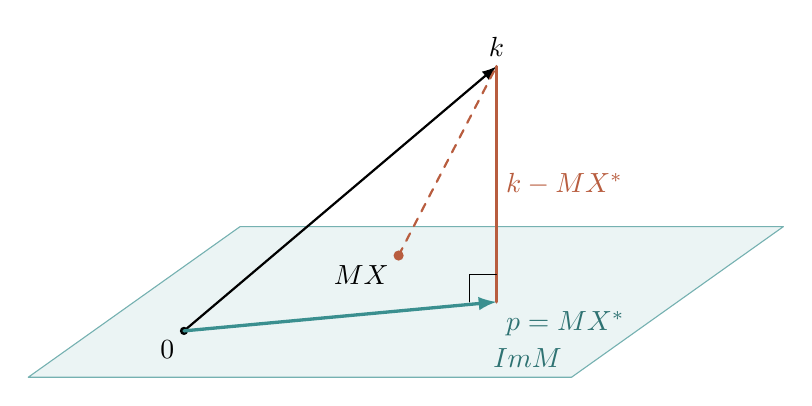
\begin{tikzpicture}[x={(1cm,0cm)}, y={(0.45cm,0.32cm)}, z={(0cm,1cm)}, line cap=round, line join=round, scale=1.15]
    \definecolor{oymteal}{RGB}{58,143,143}
    \definecolor{oymorange}{RGB}{184,93,63}
    % Plan Im M
    \fill[oymteal!10] (-1,-1.6,0) -- (5,-1.6,0) -- (5,3.6,0) -- (-1,3.6,0) -- cycle;
    \draw[oymteal!70] (-1,-1.6,0) -- (5,-1.6,0) -- (5,3.6,0) -- (-1,3.6,0) -- cycle;
    \node[oymteal!80!black, anchor=south east] at (5,-1.6,0) {$\operatorname{Im} M$};
    % Origine, projection p = MX*, point quelconque MX
    \coordinate (O) at (0,0,0);
    \coordinate (P) at (3,1,0);
    \coordinate (K) at (3,1,2.6);
    \coordinate (Q) at (1.2,2.6,0);
    \fill (O) circle (1.3pt) node[below left] {$0$};
    \draw[-latex, thick] (O) -- (K) node[above] {$k$};
    \draw[-latex, very thick, oymteal] (O) -- (P);
    \node[oymteal!80!black, below right] at (P) {$p = MX^*$};
    % Résidu orthogonal (trait plein) et écart quelconque (tirets)
    \draw[very thick, oymorange] (P) -- (K);
    \node[oymorange, right] at (3,1,1.3) {$k - MX^*$};
    \draw[thick, dashed, oymorange] (Q) -- (K);
    \fill[oymorange] (Q) circle (1.6pt) node[below left, black] {$MX$};
    % Angle droit
    \draw (3,1,0.3) -- (2.7,1,0.3) -- (2.7,1,0);
\end{tikzpicture}
